%%%%%%%%%%%%%%%%%%%%%%%%%%%%%%%%%%%%%%%%%
% OIST Doctoral Thesis - Temporary bound version
% LaTeX Template
% Version 0.2 (2016/04/06)
%
% This version is the temporary binding version which will be submitted to the thesis examiners.
% Many features (such as double spacing) are meant for the examiners' convenience, do not modify them.
%
% Original author:
% Jeremie Gillet
%
%%%%%%%%%%%%%%%%%%%%%%%%%%%%%%%%%%%%%%%%%

%----------------------------------------------------------------------------------------
%	PACKAGES AND OTHER DOCUMENT CONFIGURATIONS
%----------------------------------------------------------------------------------------

\documentclass[12pt, oneside]{book} % 12 pt font, one-sided book style
\usepackage[a4paper, includehead, headheight=0.6cm, inner=2.5cm ,outer=2.5cm, top=2.5 cm, bottom=2.5cm]{geometry}  % Changing size of document
\usepackage[english]{babel} % The document is in English
\usepackage[utf8]{inputenc} % UTF8 encoding
\usepackage[T1]{fontenc} % Font encoding

\usepackage{graphicx} % For including images
\graphicspath{{./Images/}} % Specifies the directory where pictures are stored

\usepackage{longtable} % tables that can span several pages
\usepackage{setspace} % For using double spacing
\usepackage[bf, font=onehalfspacing]{caption} % caption: FIG in bold, 1.5 line spacing in figure and table captions
\usepackage{pdfpages} % If you want to include a pdf file of your published paper as an appendix

\usepackage{fancyhdr} % For the headers

\newcommand{\numberedchapter}{ % Preparation for numbered chapters
	\cleardoublepage % To make sure the previous headers are passed
	\lhead{\bfseries \leftmark}}% Header
\newcommand{\unnumberedchapter}[1]{ % Preparation for unnumbered chapters
	\cleardoublepage % To make sure the previous headers are passed
	\addcontentsline{toc}{chapter}{#1} % Also adds the chapter name to the Contents
	\lhead{\bfseries #1}}% Header

\usepackage{eso-pic} % For the background picture on the title page
\newcommand\BackgroundPic{%
\put(-260,-140){%
\parbox[b][\paperheight]{\paperwidth}{%
\vfill
\centering

\includegraphics[width=\paperwidth]{symbol.jpg}%
\vfill
}}}

%----------------------------------------------------------------------------------------
%	ADD YOUR CUSTOM VALUES, COMMANDS AND PACKAGES
%----------------------------------------------------------------------------------------

% Open Preamble/mydefinitions.tex and enter some values (name, thesis title...) 
% and include your own custom LaTeX functions and packages

%----------------------------------------------------------------------------------------
%	VALUES FOR THE THESIS
%----------------------------------------------------------------------------------------

\newcommand{\name}{Lee James O'Riordan} % Author name
%\newcommand{\thesistitle}{The life and death of vortex 161} % Title of the thesis
\newcommand{\thesistitle}{Non-equilibrium vortex dynamics in rapidly rotating Bose--Einstein condensates} % Title of the thesis
\newcommand{\submissiondate}{October, 2016} % Submission date "Month, year"
\newcommand{\supervisor}{Prof. Thomas Busch} % Supervisor name
%\newcommand{\cosupervisor}{C.~O'Supervisor} % Co-Supervisor name, comment this line if there is none


%----------------------------------------------------------------------------------------
%	BIBLIOGRAPHY STYLE (pick the style you want)
%----------------------------------------------------------------------------------------

\usepackage[square, numbers, sort&compress]{natbib} % for bibliography - Square brackets, citing references with numbers, citations sorted by appearance in the text and compressed (as in [4-7])
%\usepackage[longnamesfirst,round]{natbib} % Natural Sciences bibliography

\bibliographystyle{Preamble/url} % You may use a different style adapted to your field
%\bibliographystyle{unsrtnat} % You may use a different style adapted to your field
%\bibliographystyle{Preamble/mlxd} % You may use a different style adapted to your field


%----------------------------------------------------------------------------------------
%	YOUR PACKAGES (be careful of package interaction)
%----------------------------------------------------------------------------------------


\usepackage{amsthm,amsmath,amssymb,amsfonts,bbm}% Math symbols
\usepackage{flexisym,mathrsfs,cancel}
\usepackage[parfill]{parskip}
%\usepackage{tocbibind}
\PassOptionsToPackage{hyphens}{url}\usepackage{hyperref}
%\usepackage[hyphens]{url}

\usepackage{chapterbib}
\usepackage{float}


%\iffalse
%%%%%%% For stopping figures taking their own pages
\setcounter{topnumber}{2}
\setcounter{bottomnumber}{2}
\setcounter{totalnumber}{4}
\renewcommand{\topfraction}{0.85}
\renewcommand{\bottomfraction}{0.85}
\renewcommand{\textfraction}{0.15}
\renewcommand{\floatpagefraction}{0.8}
\renewcommand{\textfraction}{0.1}
\setlength{\floatsep}{10pt plus 3pt minus 3pt}
\setlength{\textfloatsep}{3ex plus 1pt minus 1pt}
\setlength{\intextsep}{10pt plus 3pt minus 3pt}

\setlength{\belowcaptionskip}{3ex plus 1pt minus 1pt}
%%%%%%%
%\fi

%DOOM

\newfontfamily\doomfontL[Path=./fonts/]{AmazDooMLeft.ttf}
\newfontfamily\doomfontR[Path=./fonts/]{AmazDooMRight.ttf}
\newfontfamily\doomfontLO[Path=./fonts/]{AmazDooMLeftOutline.ttf}

%%%

\DeclareMathOperator*{\atantwo}{atan2}
\DeclareMathOperator*{\argmin}{arg\,min}

%\DeclareMathOperator*{\textprime}{'}

\newcommand{\lee}{\textcolor{red}}
\usepackage{todonotes}
\usepackage{subcaption}
\usepackage{braket} %useful to type directly diacritic characters
\usepackage{algpseudocode}
%\usepackage{xeCJK}
%\setCJKmainfont{MS Mincho} % for \rmfamily
%\setCJKsansfont{MS Gothic} % for \sffamily
%\usepackage{unicode-math}
%\setmathfont{xits-math.otf}


%\usepackage[utf8]{inputenc}
%----------------------------------------------------------------------------------------
%	YOUR DEFINITIONS AND COMMANDS
%----------------------------------------------------------------------------------------

% New Commands
    \renewcommand{\baselinestretch}{1.2}


\newcommand{\bea}{\begin{eqnarray}} % Shortcut for equation arrays
\newcommand{\eea}{\end{eqnarray}}
\newcommand{\e}[1]{\times 10^{#1}}  % Powers of 10 notation

% Defining a theorem box for Criteria
\newtheorem{critere}{Criterion}
\newcommand{\crit}[2]{
\begin{center}
\fbox{ \begin{minipage}[c]{0.9 \textwidth}
\begin{critere}
\textbf{\textup{ #1}} --- #2
\end{critere}
\end{minipage}  } \end{center}
}


\begin{document}

%----------------------------------------------------------------------------------------
%	TITLE PAGE
%----------------------------------------------------------------------------------------

\pagestyle{empty} % No page numbers
\frontmatter % Use roman page numbering style (i, ii, iii, iv...) for the preamble pages

\begin{titlepage}
\AddToShipoutPicture*{\BackgroundPic}
\begin{center}
\vfill
{\large \scshape Okinawa Institute of Science and Technology\\Graduate University}\\[0.7cm]
{\large Thesis submitted for the degree }\\[0.7cm]
{\Large Doctor of Philosophy}\\[0.5cm]
\rule{\textwidth}{1.5pt}\\[0.5cm]
{\huge \bfseries \thesistitle}\\[0.5cm]
\rule{\textwidth}{1.5pt}\\[2.5cm]
\hfill  by\\[1cm]
\hfill  {\large \bfseries\name}\\
\vfill
{\hfill \large Supervisor: \textbf{\supervisor}} \\ 
\ifx\cosupervisor\undefined\else{\hfill \large Co-Supervisor: \textbf{\cosupervisor}} \\ \fi
\vspace{1cm}
\hfill  \submissiondate
\end{center}
\end{titlepage}

%----------------------------------------------------------------------------------------
%	PREAMBLE PAGES (delete unnecessary pages)
%----------------------------------------------------------------------------------------

\pagestyle{fancy} % Change the header style
\fancyhf{}% Clear header and footer
\renewcommand{\chaptermark}[1]{\markboth{#1}{}} % Getting the chapter name right
\rhead{\thepage} % Page number at the right of the header
\frontmatter % Use roman page numbering style (i, ii, iii, iv...) for the preamble pages
\setcounter{page}{2} % Include the title page in page counting
\doublespacing % Double spacing

\unnumberedchapter{Declaration of Original and Sole Authorship} 
\chapter*{Declaration of Original and Sole Authorship} 

I, \name, declare that this thesis entitled \emph{\thesistitle} and the data presented in it are original and my own work. 


I confirm that:
\begin{itemize}
\item This work was done solely while a candidate for the research degree at the Okinawa Institute of Science and Technology Graduate University, Japan.
\item No part of this work has previously been submitted for a degree at this or any other university.
\item References to the work of others have been clearly attributed. Quotations from the work of others have been clearly indicated, and attributed to them.
\item In cases where others have contributed to part of this work, such contribution has been clearly acknowledged and distinguished from my own work.
\item None of this work has been previously published elsewhere, with the exception of the following: (provide list of publications or presentations, or delete this part). 
(If the work of any co-authors appears in this thesis, authorization such as a release or signed waiver from all affected co-authors must be obtained prior to publishing the thesis.  If so, attach copies of this authorization to your initial and final submitted versions, as a separate document for retention by the Graduate School, and indicate on this page that such authorization has been obtained).  
\end{itemize}

Date:  \submissiondate

Signature: 

\unnumberedchapter{Abstract}
\chapter*{Abstract}
\subsection*{\thesistitle}

This body of work examines the non-equilibrium dynamics of vortex lattice carrying Bose--Einstein condensates. We solve the mean-field Gross--Pitaevskii equation for a two-dimensional pancake geometry, in the co-rotating frame within the limit of high rotation frequencies. The condensate responds to this by creating a large periodic lattice of vortices with 6-fold triangular symmetry. By applying two distinct perturbations to this lattice, we examine the resulting effects on the vortices during time evolution. The first perturbation involves applying an optical potential with matching geometry to the vortex lattice. We observe the appearance of interference fringes, and we show that these can be described by moir\'e interference theory. This is backed up by a decomposition of the kinetic energy spectra of the condensate. The applied perturbation only modifies the condensate density, with the vortex positions largely unaffected. From this we conclude that the vortex lattice is very stable and robust against phononic disturbances.

Next, by removing vortices at predefined positions in the lattice using phase imprinting techniques, we examine the resulting order of the lattice. By performing this we generate stable topological defects in the crystal structure.  The resulting lattice remains highly ordered in the presence of low numbers of these defects, where crystal structure and order of the lattice shows to be highly robust. By varying the type of imprinted phases we can create controllable degrees of disorder in the lattice. This disorder is analysed using orientational correlations, Delaunay triangulation, and Voronoi diagrams of the vortex lattice, and demonstrates a method for examining order and generating disorder in vortex lattices in Bose--Einstein condensates.

All work described makes extensive use of GPU computing techniques, and allows for the simulation of these systems to be realised in short times. The implementation of the calculations using GPU computing are also discussed, where the software is shown to be the fastest of its kind out of the independently tested software suites. 

\unnumberedchapter{Acknowledgment}
\chapter*{Acknowledgments}

%\begin{figure}[h!]\centering
%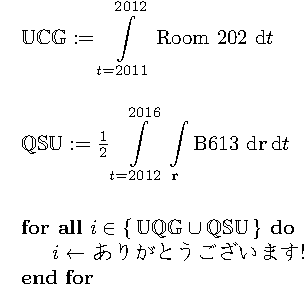
\includegraphics[width=0.4\textwidth]{Preamble/ack_stand/ack_stand}
%\vspace{1ex}
%\end{figure}
%\begin{lstlisting}[breaklines]
$/*$
Firstly, I would like to express my sincerest gratitude to my family back in the 'mel who have always been there for me, and provided amazing support from across the planet since I started my PhD (and before I started too) --- most notably, to Mum, Nan and Maria, who have done so much over the years. Next, my sincerest gratitude and thanks goes to Prof. Thomas Busch, for freeing me from the shackles of a boring job and introducing me to the (ultra)cool world of atomic physics, as well as the guidance he has offered over the years. To past and present members of both the Ultracold Quantum Gases group at University College Cork, and Quantum Systems Unit at OIST, thanks for keeping me sane and helping out through the work and writing over the years --- in no particular order: Mossy, Steve, Jeremie, Tara, Albert, Angela, Sawako, Rashi, James, Irina, the magnificent Dave Rea, and of course Tadhg. Next, I would like to thank the Graduate School for all of their help removing bureaucratic dealings from my everyday life here. A special thanks also goes to the Scientific Computing Section, for allowing me access to some very amazing toys over these past few years. A special thanks also to Annie, for supplying me with enough caffeine to get to the moon and back. Lastly, but not least-ly, to Christina for her compassion, understanding, and assistance over the past few years. $*/$
%\end{lstlisting}


\begin{algorithmic}
\ForAll{$i \in \{S | S \in \textrm{People to thank} \}$}
    \State $i\gets$ ありがとうございます!
\EndFor
\end{algorithmic}

\unnumberedchapter{Abbreviations} 
\chapter*{Abbreviations} 

All abbreviations used in the thesis should be listed here, with their definitions, in alphabetical order.  This includes trivial and commonly used abbreviations (at your own discretion), but not words that have entered into general English usage (such as laser or DNA).  In particular, non-standard abbreviations should be presented here.  This is an aid to the reader who may not read all sections of the thesis. \\ % You can delete this paragraph, only the table is needed.

\begin{longtable}{rl}
PPT & positive partial transpose\\
SRPT & Schr\"odinger-Robertson partial transpose
\end{longtable}
\unnumberedchapter{Glossary} 
\chapter*{Glossary} 

% Break up this table into several ones if it takes up more than one page
\begin{center}
\begin{longtable}{r p{0.58 \textwidth}}
Chemical potential & Energy to overcome for adding an atom to the system
\end{longtable}
\end{center}

\unnumberedchapter{Nomenclature} 
\chapter*{Nomenclature} 

% Break up this table into several ones if it takes up more than one page
\begin{longtable}{rl}
$h$ & Planck constant ($6.626\ 070\ 04\e{-34}\ \mbox{Js}$). \\
$\hbar$ & Planck constant over $2\pi$ ($1.054\ 572\ 66\e{-34}\ \mbox{Js}$). \\
$L_z$ & Angular momentum operator along the $z$-dimension; $xp_y-yp_x$. \\
$\nabla$ & Gradient operator. \\
$\Omega$ & Angular rotation frequency of condensate. \\
$\xi$ & Condensate healing length; the distance from a region of zero density at vortex core to bulk density. \\
$\mu$ & Chemical potential of the condensate; the energy change per unit change in particle number. \\
\end{longtable}
\cleardoublepage
\thispagestyle{empty} % Page style needs to be empty for this page

\vspace*{8cm} 

\hfill
\begin{parbox}{0.6\textwidth}{
\begin{flushright}

If desired, an optional and short dedication may be included here.

\end{flushright}}
\end{parbox}




%----------------------------------------------------------------------------------------
%	LIST OF CONTENTS/FIGURES/TABLES
%----------------------------------------------------------------------------------------

\unnumberedchapter{Contents}
\tableofcontents % Write out the Table of Contents
\unnumberedchapter{List of Figures}
\listoffigures % Write out the List of Figures
\unnumberedchapter{List of Tables}
\listoftables % Write out the List of Tables

%----------------------------------------------------------------------------------------
%	THESIS MAIN TEXT
%----------------------------------------------------------------------------------------

\addtocontents{toc}{\vspace{2em}} % Add a gap in the Contents, for aesthetics
\mainmatter % Begin numeric (1,2,3...) page numbering

\unnumberedchapter{Introduction} % Title of the unnumbered chapter
%\chapter*{Introduction}  % Name of the unnumbered section

This body of work was carried out during my time as a Ph.D student at Okinawa Institute of Science and Technology Graduate University (OIST). The purpose of the work described herein was to understand the dynamics of rapidly rotating Bose--Einstein condensates subjected to perturbations. While it is possible derive some analytical solutions to rapidly rotating condensate behaviour (LLL), such solutions are rare. This thesis concentrates on the numerical solutions of the Gross--Pitaevskii equation, and the resulting dynamics of those solutions.

This work is motivated by the use of Bose--Einstein condensate (BEC) systems as model tools to investigate turbulent and chaotic quantum behaviour. Ideally, these systems can also be used for long-term memory storage for quantum computing systems. Finally, these type of systems allow the study of quantum mechanical effects on mesoscopic scales, making them a great tool for simulating condensed matter physics. Given these statements, being able to manipulate and engineer specific states, and thus behaviour, from BECs requires tools to allow this. I investigate the use of kicked optical potentials and direct phase engineering of the wavefunction and examine their usefulness for generating such behaviour.

To do this we assume a trial system of a BEC rapidly rotating to generate a large number of vortices, arranged in a triangular pattern pattern. The trial wavefunction is subjected to the different manipulations listed earlier, and I examine the resulting dynamics. A large numerical component will be required to perform such simulations, and so I will also discuss the development of numerical tools using graphics processing units (GPU) for these studies, with comparisons drawn against standard simulation techniques.

The thesis will be outlined as follows:

\section{Chapter 1}
The field of cold-atomic gas systems will be introduced, and the theory of Bose--Einstein condensation discussed. The field will be thoroughly examined and discussed via a literature review, examining theory, experimentation, origins and also future of the field. Emphasis will be placed on material and works relevant to the study performed herein.

\iffalse
Introduction (~5-10 pages)

    - Thesis Statement (one or two sentences)
        What is your thesis about and what have you done?
        If you have a hypothesis what is it?
        How will you test (prove/disprove) your hypothesis?
    - Motivation
        Why is this problem you've worked on important
    - Goals / Objectives
        What are you trying to do and why?
        How will you or the reader know if or when you've met your objectives?
    - **** Contributions *****
        What is new, different, better, significant?
        Why is the world a better place because of what you've done?
        What have you contributed to the field of research?
        What is now known/possible/better because of your thesis?
    Outline of the thesis (optional)
\fi

\section{Chapter 2}
    Here I examine the use of methods for describing the Bose--Einstein condensate numerically. I introduce the necessary algorithms and considerations to simulate such a system. General purpose GPU (GPGPU) computing will be introduced here, with the implementation of the Gross--Pitaevskii equation discussed. Calculation of the Bogoloiubov spectrum, and its implementation is discussed here also.

\iffalse
Background / Related Work (~8-20 pages)
    More than a literature review
    Organize related work - impose structure
    Be clear as to how previous work being described relates to your own.
    The reader should not be left wondering why you've described something!!
    Critique the existing work - Where is it strong where is it weak? What are the unreasonable/undesirable assumptions?
    Identify opportunities for more research (i.e., your thesis) Are there unaddressed, or more important related topics?
    After reading this chapter, one should understand the motivation for and importance of your thesis
    You should clearly and precisely define all of the key concepts dealt with in the rest of the thesis, and teach the reader what s/he needs to know to understand the rest of the thesis.
\fi

\section{Chapter 3}
\iffalse
Theory / Solution / Program / Problem (~15-30 pages)

    continuing from Chapter 2 explain the issues
    outline your solution / extension / refutation
\fi

\section{Chapter 4}

\iffalse Implementation / Formalism (~15-30 pages)
    not every thesis has or needs an implementation
\fi

\section{Chapter 5}

\iffalse
Results and Evaluation (~15-30 pages)

    adequacy, efficiency, productiveness, effectiveness (choose your criteria, state them clearly and justify them)
    be careful that you are using a fair measure, and that you are actually measuring what you claim to be measuring
    if comparing with previous techniques those techniques must be described in Chapter 2
    be honest in evaluation
    admit weaknesses
\fi

\section{Chapter 6}
\iffalse
 Conclusions and Future Work (~5-10 pages)

    State what you've done and what you've found
    Summarize contributions (achievements and impact)
    Outline open issues/directions for future work
\fi
 % Introduction (unnumbered)

\numberedchapter % Regular chapters following
\input{MainText/chapter1} % Input your chapters here
\input{MainText/chapter2} 
\input{MainText/chapter3} 
%\input{MainText/chapter4} 
%\input{MainText/chapter5} 

\unnumberedchapter{Conclusion} % Title of the unnumbered chapter
\chapter*{Conclusion}  % Name of the unnumbered section

This is the conclusion. You might want to leave it unnumbered, as it is now. If you want to number it, treat it like any other chapter. % Conclusion (unnumbered)

%----------------------------------------------------------------------------------------
%	APPENDICES
%----------------------------------------------------------------------------------------
\addtocontents{toc}{\vspace{2em}} % Add a gap in the Contents, for aesthetics
\appendix 

\numberedchapter % Regular chapters following


\chapter{Appendices and Supplementary Data} \label{appA}

Unlike a journal article, no data or discussion may be presented separately as unpublished supplementary documents or data.  Appendices should be used instead for material that is tangentially relevant to the thesis but does not fit in the main narrative. If you need to refer to large volumes of data that cannot be printed (such as an annotated genome, or a simulation with moving images), lodge the data on an OIST repository or a public database and provide the URL of the dataset in the thesis.  

%\input{MainText/appendixB}
%\input{MainText/appendixC}

%----------------------------------------------------------------------------------------
%	BIBLIOGRAPHY
%----------------------------------------------------------------------------------------

\addtocontents{toc}{\vspace{2em}} % Add a gap in the Contents, for aesthetics
\unnumberedchapter{Bibliography} % Title of the unnumbered chapter
\bibliography{Preamble/Thesis_bibliography} % The references information are stored in the file named "Thesis_bibliography.bib"

%----------------------------------------------------------------------------------------
%	PUBLISHED ARTICLES - ONLY INCLUDE PDF FILES HERE
%----------------------------------------------------------------------------------------

\addtocontents{toc}{\vspace{2em}} % Add a gap in the Contents, for aesthetics
\unnumberedchapter{Published articles} % Title of the unnumbered chapter
\chapter*{Published articles} % Starts a chapter which will remain empty


\includepdf[pages=-, offset=0.54cm \voffset]{./Images/papers/ch01_who-we-are_en_20151028_cl.pdf} % Includes pdf
%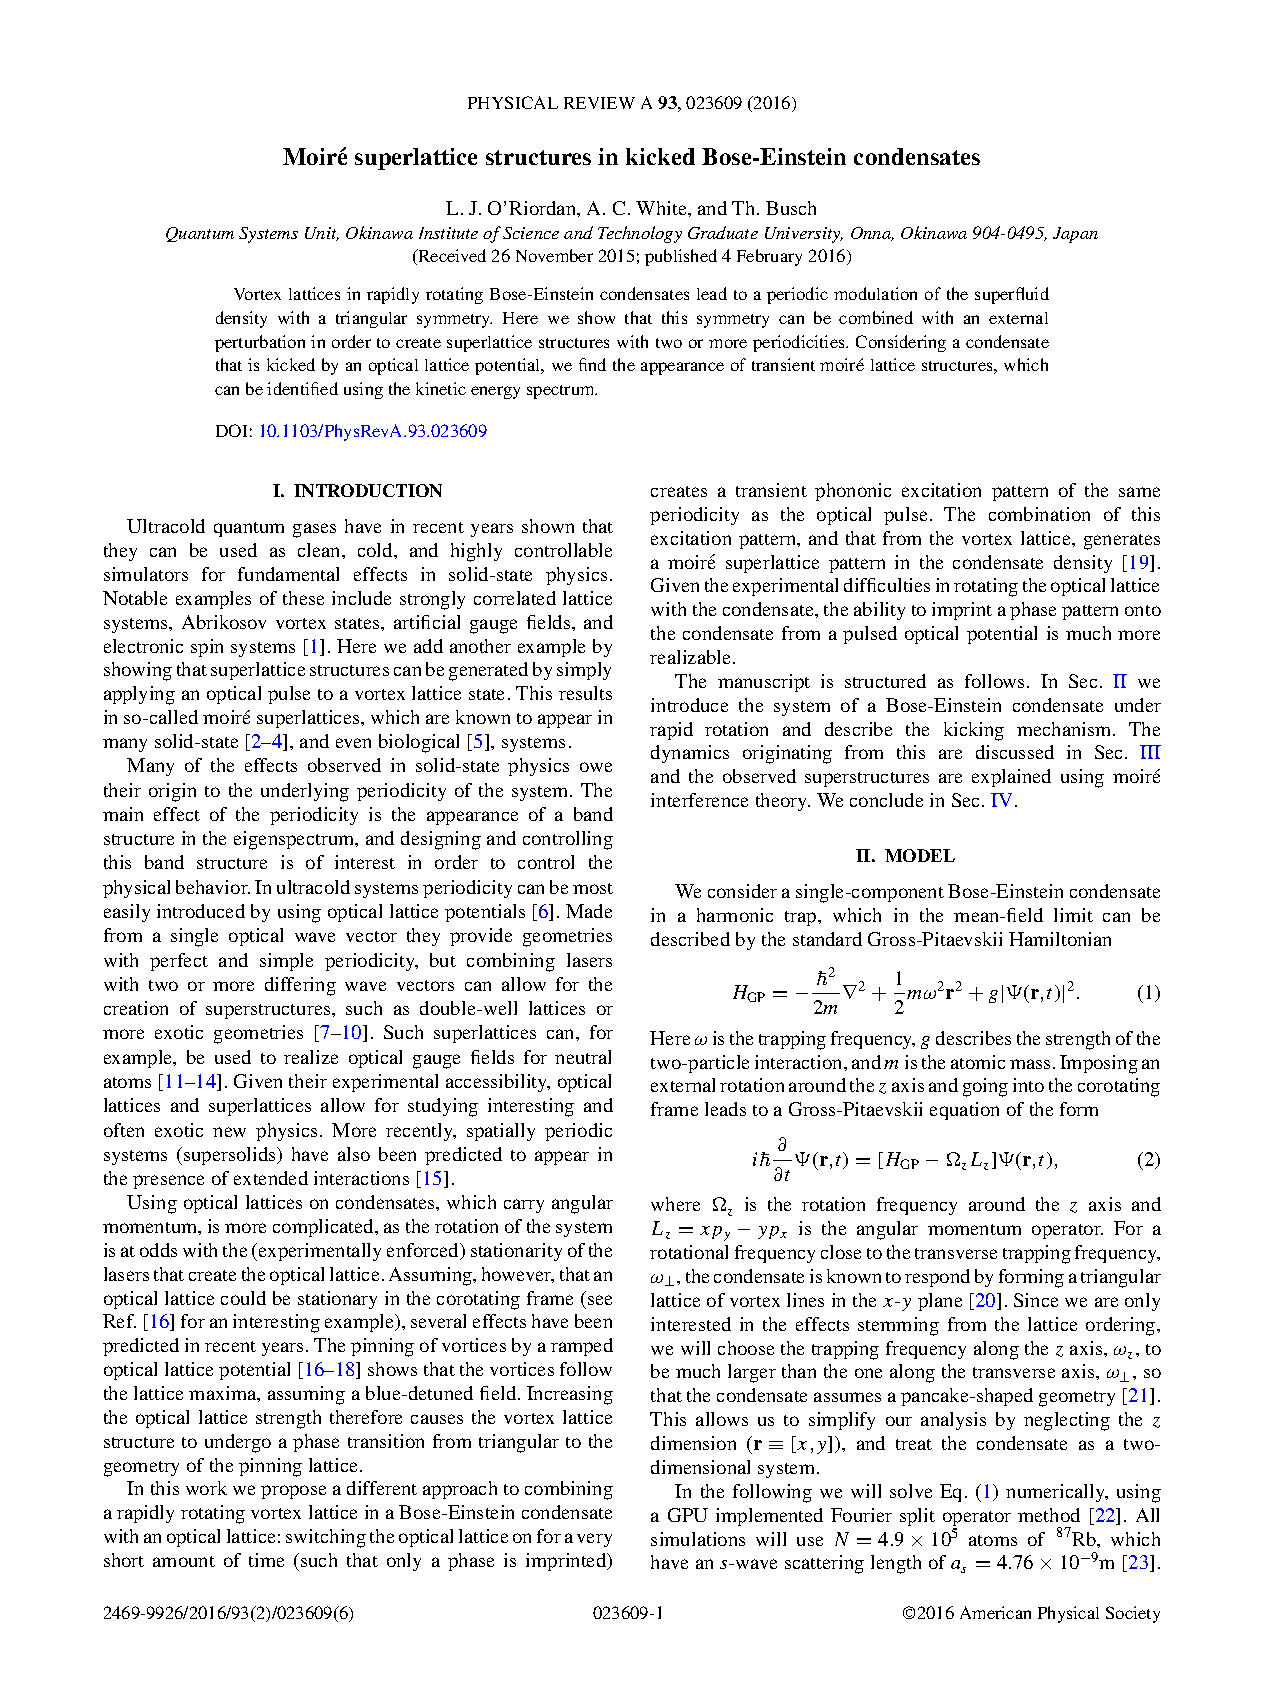
\includepdf[pages=-, offset=0.54cm \voffset]{./Images/papers/paper2.pdf} % Includes pdf
%\includepdf[pages=-, offset=0.54cm \voffset]{./Images/papers/paper3.pdf} % Includes pdf

\end{document}  